%iffalse
\let\negmedspace\undefined
\let\negthickspace\undefined
\documentclass[journal,12pt,twocolumn]{IEEEtran}
\usepackage{cite}
\usepackage{amsmath,amssymb,amsfonts,amsthm}
\usepackage{algorithmic}
\usepackage{graphicx}
\usepackage{textcomp}
\usepackage{xcolor}
\usepackage{txfonts}
\usepackage{listings}
\usepackage{enumitem}
\usepackage{mathtools}
\usepackage{gensymb}
\usepackage{comment}
\usepackage[breaklinks=true]{hyperref}
\usepackage{tkz-euclide} 
\usepackage{listings}
\usepackage{gvv}                                        
%\def\inputGnumericTable{}                                 
\usepackage[latin1]{inputenc}                                
\usepackage{color}                                            
\usepackage{array}                                            
\usepackage{longtable}                                       
\usepackage{calc}                                             
\usepackage{multirow}                                         
\usepackage{hhline}                                           
\usepackage{ifthen}                                           
\usepackage{lscape}
\usepackage{tabularx}
\usepackage{array}
\usepackage{float}


\newtheorem{theorem}{Theorem}[section]
\newtheorem{problem}{Problem}
\newtheorem{proposition}{Proposition}[section]
\newtheorem{lemma}{Lemma}[section]
\newtheorem{corollary}[theorem]{Corollary}
\newtheorem{example}{Example}[section]
\newtheorem{definition}[problem]{Definition}
\newcommand{\BEQA}{\begin{eqnarray}}
\newcommand{\EEQA}{\end{eqnarray}}
\newcommand{\define}{\stackrel{\triangle}{=}}
\theoremstyle{remark}
\newtheorem{rem}{Remark}

% Marks the beginning of the document
\begin{document}
\bibliographystyle{IEEEtran}
\vspace{3cm}

\title{1.2.14}
\author{EE24BTECH22053 - S A Aravind Eswar}
\maketitle
\newpage
\bigskip

\renewcommand{\thefigure}{\theenumi}
\renewcommand{\thetable}{\theenumi}

\textbf{Question:}Verify if the points \textbf{A}(4, 3), \textbf{B}(6, 4), \textbf{C}(5, -6) and \textbf{D}(-3, 5) are the vertices of a
parallelogram.\\
\solution 
\begin{table}[h]
	\centering
	\begin{tabular}{|m{5em} | m{7em} | m{10em} |}
    \hline
    \textbf{symbol} & \textbf{Value} & \textbf{Description}\\
    \hline
        \textbf{V},\textbf{u},f & $\myvec{ 1 & 0\\0 & 0}$, $\myvec{0\\2}$, 0 & Parameters of the given conic (parabola)\\
    \hline
        $\vec{h_1}, \vec{m_1}$ & $\myvec{0\\2}, \myvec{1\\0}$ & Parameters of the given line $y = 2$\\
    \hline
        $\vec{h_2}, \vec{m_2}$ & $\myvec{0\\4}, \myvec{1\\0}$ & Parameters of the given line $y = 4$\\
    \hline
        $\vec{a_1}, \vec{a_2}$ & & Points of intersection of given lines to the conic\\
    \hline
        $\kappa_i$ & & Parameters of the line equation $\vec{x} = \vec{h} + \kappa\vec{m}$\\
    \hline
        $A_1$ & & Area under the parabola from $y=0$ to $y=4$\\
    \hline
        $A_2$ & & Area under the parabola from $y=0$ to $y=2$\\
    \hline
\end{tabular}

	\caption{Given Values}
	\label{tab:1}
\end{table}

For points \textbf{A},\textbf{B},\textbf{C} and \textbf{D} to form a parallelogram, we'll need 2 vectors formed by different points to be equivalent.
\begin{align*}\textbf{AB} &= \textbf{B}-\textbf{A} &= \myvec{2\\1}\\\textbf{BC} &= \textbf{C}-\textbf{B} &= \myvec{-1\\-10}\\\textbf{CD} &=\textbf{D}-\textbf{C} &=\myvec{-8\\11}\\\textbf{DA} &= \textbf{A}-\textbf{D} &= \myvec{7\\-2}\\\textbf{BD} &= \textbf{D}-\textbf{B} &= \myvec{-9\\1}\\\textbf{AC} &= \textbf{C}-\textbf{A} &= \myvec{1\\-9}\\\end{align*}
But here, we see no such possibility arising with the vectors. And thus, the points \textbf{A},\textbf{B},\textbf{C} and \textbf{D} are not forming a parallelogram.


\begin{figure}[h]
    \centering
    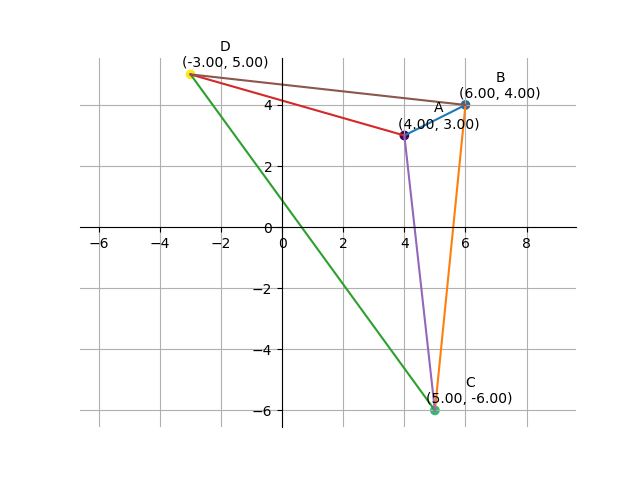
\includegraphics[width=\columnwidth]{figs/fig1.png}
    \caption{Points \textbf{A},\textbf{B},\textbf{C} and \textbf{D}}
 \end{figure}

\end{document}
